\subsection{Current and Previous Solutions}
\label{description:solution}
Currently Tomboy has the functionality to create bullet lists in Notes and with help of the Backlink Addin (which is shipped with the default Tomboy installation) to add Hyperlinks between different Notes. This allows the user to create simple task lists through Bulletlist and through linking a single task to another Note to create subtasks. This functionality is also shown in the GUI Mockup in Figure \ref{gui}.

In the past, there have been several official and inofficial attempts to come up with an Addin for handling tasks in Tomboy which however all did not result in a satisfactory end product due to missing functionality or integration. Our goal is to implement such a project up to a stable and working solution that, such that it could be included in the Tomboy project and shipped with future Tomboy releases. 

\label{lessons}
Since those earlier projects directly influenced some of our design decisions with respect to \textit{bug-freeness}, \textit{usability} and \textit{integration into Tomboy}, section \ref{appendix} goes into detail about some of those projects and why they failed to achieve their requirements.

\subsection{Product Perspective}
\label{description:perspective}
  The project TaskManager for Tomboy will be part of the Tomboy project. There will be three main interfaces:

  \begin{itemize}
    \item The first one is the obvious user interface that the user sees within Tomboy.
    \item The representation of our data will be integrated in Tomboy Note files. That means, persistent storage of the Tasks must be accomplished as XML files using the structures already existing.
    %TODO: Mention this structure
    \item Exporting data, to be read from/to other note taking applications. Will be done using XML.
  \end{itemize}

  Figure \ref{perspective} shows the Product perspective of the TaskManager Addin. Since it's really an extension for the Tomboy Application it is placed in Tomboy itself where it will communicate with some of Tomboys internal elements (as shown by arrows). Further the Addin will rely directly on some of the GTK\# Widgets.
  \begin{figure}[ht]
    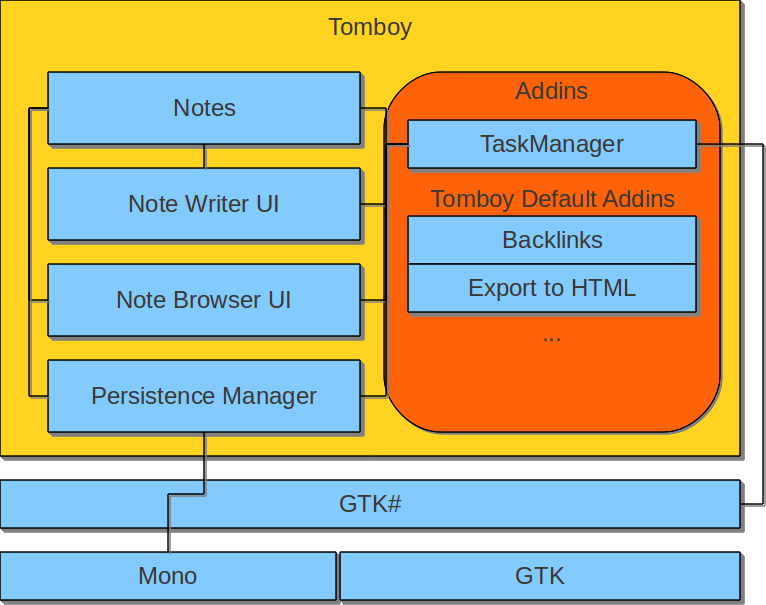
\includegraphics[width=\textwidth]{graphics/product_perspective_diagram.png}
    \caption{TaskManager Product Perspective}
    \label{perspective}
  \end{figure}


\subsection{Product Functions}
\label{description:functions}

  \subsubsection*{Supported Functions}
  \label{description:functions:supported}

    \begin{itemize}
      \item Provides advanced Task management capabilities for Tomboy
      \item Allows multiple tasks to be grouped together
      \item Supports priorities and due dates for tasks
      \item Allows to establish relationships/dependencies between tasks
      %TODO: v Is this really one of the core functionalities that we can guarantee to implement? v
      \item Allows the user to conveniently get to the tasks currently not finished/finished or overdue.
      \item Allows to export all defined tasks
    \end{itemize}

    \subsubsection*{Unsupported Functions}
      \label{description:functions:unsupported}
      \begin{itemize}
        \item Does not introduce additional GUI window elements or external tools within or outside of Tomboy (see \ref{lessons}).
        \item Does not support on-the-fly synchronization with external tools or clients except for manual export.
        \item Does not support importing tasks from other Task manager tools.
      \end{itemize}

\subsection{User Characteristics}
\label{description:usercharacteristics}
We look at two types of users:

  \begin{itemize}
    \item[\bf{Casual}] The casual user will create simple task lists. He may not know the various functions of Tomboy very well. Still, he will be able to create simple task lists where he can cross out individual elements easily.

    \item[\bf{Advanced}] The advanced user knows and uses Tomboy already quite well. He is able to add arguments such as due dates and priorities to his task lists, create hierarchies of tasks and may export his lists to other tools such as \textit{Evolution} without much effort.
    %TODO: Is there really ONE output format that allows this?

  \end{itemize}


\subsection{Constraints}
\label{description:constraints}
%TODO: Recheck example requirements document: Are those two sections really redundant?
The Addin itself will obey all criterias (standards and guidelines) imposed by the GNOME and Tomboy projects (Tomboy Styleguide, \ref{styleguide}).

Besides the coding guidelines this includes mainly design aspects, such as simplicity and easyness of use, and full integration into Tomboy (see also \ref{integration}).


\subsection{Assumptions and Dependencies}
\label{description:assumptions}
